\documentclass{article}
\usepackage{graphicx}
\usepackage{caption}
\usepackage{subcaption}
\usepackage{amsmath}
\newcommand{\kcat}{$k_\mathrm{cat}$ }
\newcommand{\rcat}{$r_\mathrm{cat}$ }
\newcommand{\rmax}{$r_\mathrm{cat}^\mathrm{max}$ }
\newcommand{\vmax}{$v_\mathrm{max}$}
\newcommand{\vmin}{$v_\mathrm{min}$}
\begin{document}

\section*{Estimating the errors in \rcat}

Regarding the errors in the \textit{in vitro} \kcat measurements,  it is not clear how to introduce the errors in  as in many cases, values measured for the same enzymes are measured using different methods and under different conditions.
\subsection*{Methodological Errors in \kcat are }
\subsection*{Flux Variability Analysis}
One of the main concerns in our approach for calculating the maximal catalytic rate of an enzyme, is how to get a representative flux value to plug in the equation:
\begin{align}
r_\mathrm{cat} &= \frac{v_i}{E_i} 
\end{align}
Currently, we solve parsimonious FBA (pFBA), which minimizes the total sum of fluxes. It was shown that pFBA agrees with trnascriptional data from E. coli in 97\% of the time, and is considered a reasonable approch from flux predictions among the FBA community.\\
However, the flux values we get for each reaction are random sample from a possible flux distribution and may not represent the "real" flux through a given reaction. To reduce biases in our \rcat estimations, we can consider parsimonious \emph{FVA}, which returns a range of fluxes for each reaction. It works in the following manner:
\begin{align*}
&(1)\text{ solve pFBA} \\
&(2)\text{ set all reaction boundaries accordingly} \\
&(3)\text{ for each reaction in the model:} \\
&~~~~ (3a)\text{ minimize the reaction flux } (v_\mathrm{min}) \\
&~~~~ (3b)\text{ maximize the reaction flux } (v_\mathrm{min}) \\
\end{align*}

The range of flux for reaction $i$ is then:
\begin{align}
v_{\mathrm{max}, i} - v_{\mathrm{min}, i} \\
\end{align}

Taking the mean of the $v$ range may be a better approach for \rcat estimations. Error bars (or more precisely, confidence intervals) can be described as:

\begin{align}
\overline{r_{\mathrm{cat}, i}} &= \frac{v_{\mathrm{max}, i}}{E_i} \\
\underline{r_{\mathrm{cat}, i}} &= \frac{v_{\mathrm{min}, i}}{E_i} \\
\end{align}

\begin{figure}
	\center
	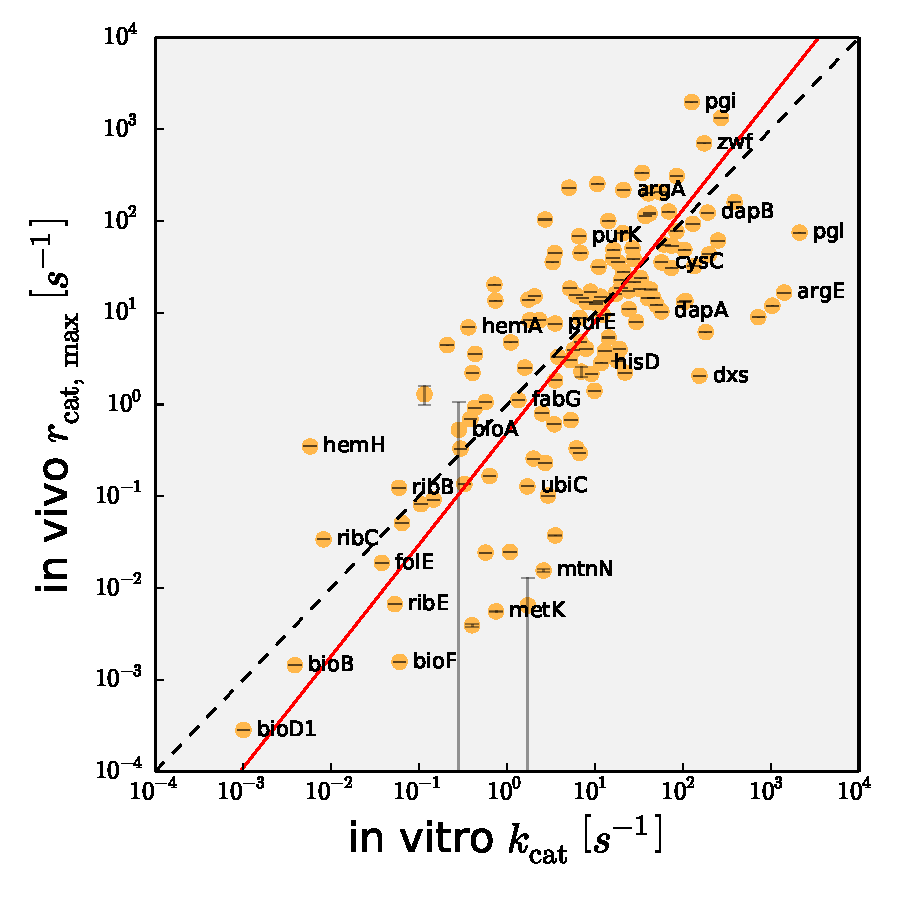
\includegraphics[width=0.8\textwidth]{../figures/kcat_to_rmax_relaxting_1_000.pdf}
	\caption{\kcat to \rmax correlation using $v_\mathrm{mean}$ as flux value for \rmax calculation. Dashed black line 	represents $y=x$ and red line represents best fit by orthogonal regression. correlation: $r^2 = 0.556$, $p_{val} < 10^{-24}$, $\mathrm{rmse} = 0.6$}
	\label{fig:pFVA}
\end{figure}

Most of our reactions seem to have a very small dynamic range of fluxes, resulting in almost zero flux-associated errors (figure \ref{fig:pFVA}). Usually, if a reactions have small flux variability it means that they are biomass related, thus must support a given amount of flux to allow growth. Nevertheless, this is not the case for most of the 135 reactions we analyze (or at least I cannot see how they are biomass related). It is possible that the minimization of fluxes constrain, on top of the other constrains (growth rate and oxygen uptake rate) leave very little room for flux deviations. We can further relax the parsimonious constraint, that is, allow the sum of fluxes to be $x\%$ larger. A common relaxing factor is in the range of 0.1-5\%. Figure \ref{fig:relax} 

\begin{figure}
        \center
        \begin{subfigure}[b]{0.3\textwidth}
                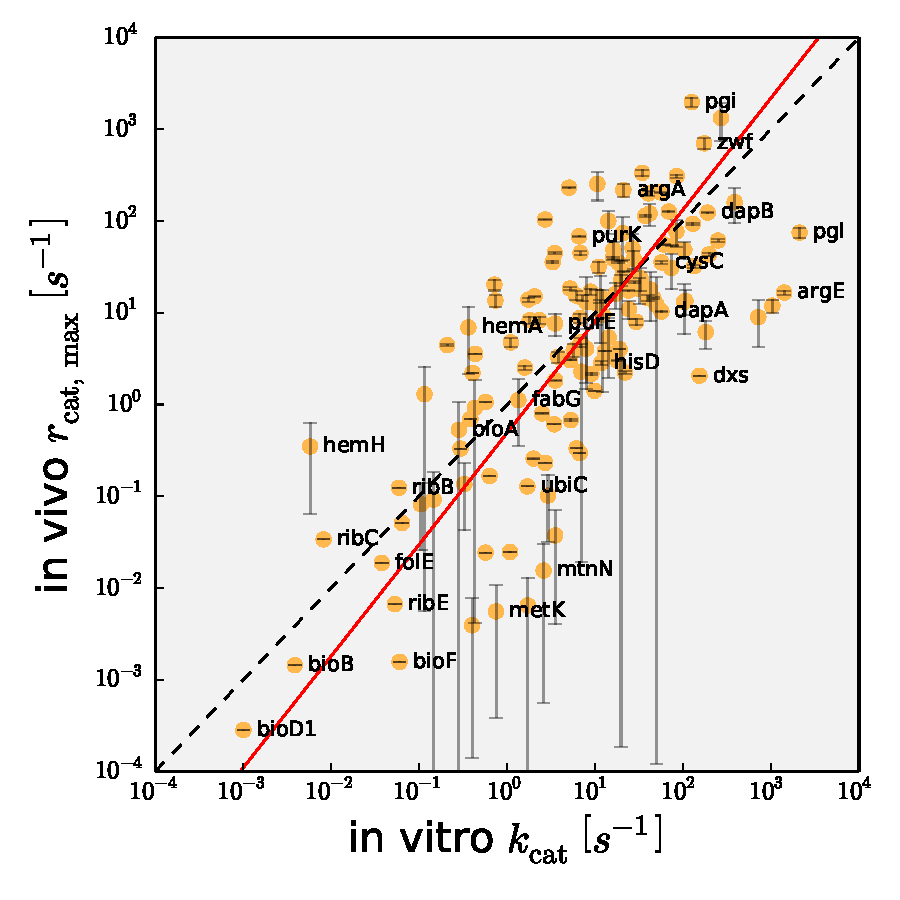
\includegraphics[width=\textwidth]{../figures/kcat_to_rmax_relaxting_1_001.pdf}
                \caption{relaxation = 0.1\%}
        \end{subfigure}%
        ~ %add desired spacing between images, e. g. ~, \quad, \qquad, \hfill etc.
          %(or a blank line to force the subfigure onto a new line)
        \begin{subfigure}[b]{0.3\textwidth}
                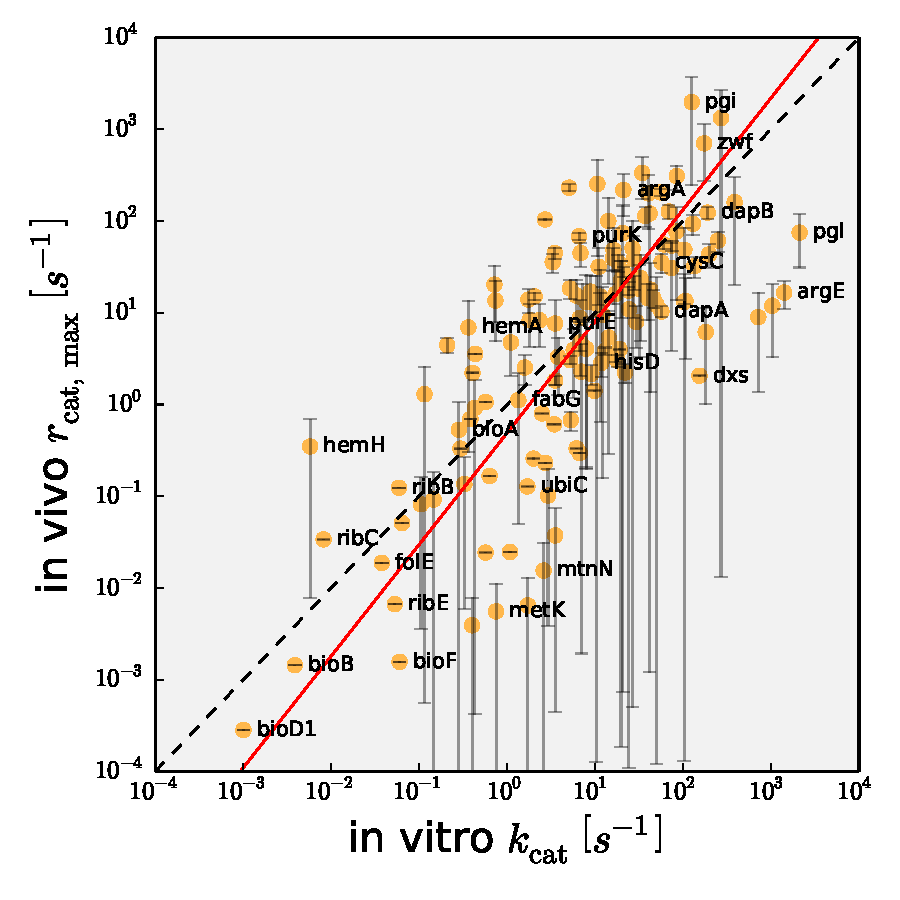
\includegraphics[width=\textwidth]{../figures/kcat_to_rmax_relaxting_1_010.pdf}
                \caption{relaxation = 1\%}
        \end{subfigure}
        ~ %add desired spacing between images, e. g. ~, \quad, \qquad, \hfill etc.
          %(or a blank line to force the subfigure onto a new line)
        \begin{subfigure}[b]{0.3\textwidth}
                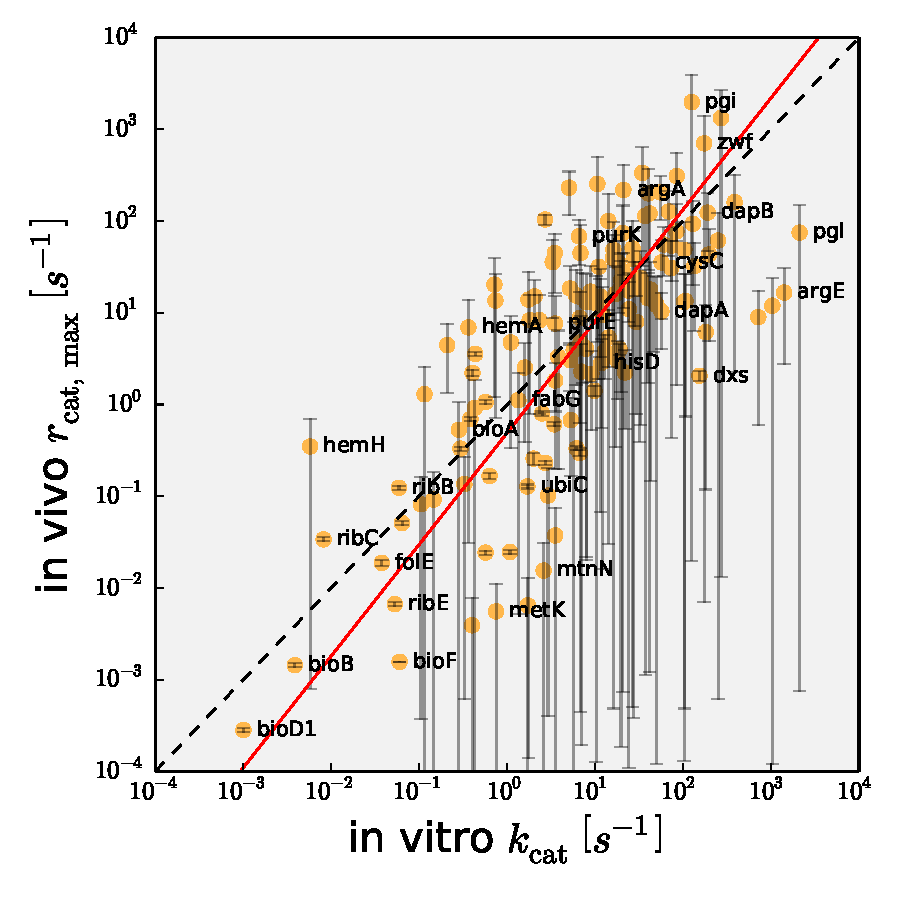
\includegraphics[width=\textwidth]{../figures/kcat_to_rmax_relaxting_1_100.pdf}
                \caption{relaxation = 10\%}
        \end{subfigure}
	\caption{}
	\label{fig:relax}	
\end{figure}

\subsection*{Standard deviation of the maximum}

We can ask how reliable \rmax is. It may be that the maximal catalytic rate across all conditions. For example if the enzyme copy number in a particular condition was reported to be extremely small, \rmax will be disproportionally high. For this, we can calculate the standard deviation of the top three \rcat values:

\begin{align*}
\mathrm{std}([r_{max}^{1st}, r_{max}^{2nd}, r_{max}^{3rd}]),
\end{align*}

Figure \ref{fig:std}a  shows the resulting error bars. A reason for such large deviations is that the catalytic rate of many enzymes is log normal distributed, thus taking the $\mathrm{std}$ of the data results in huge errors.
We can consider using:

\begin{align*}
\mathrm{std}(\log([r_{\max}^{1st}, r_{\max}^{2nd}, r_{\max}^{3rd}])),
\end{align*}

yet then the errors are very small as we are only using three numbers (fig \ref{fig:std}b).

\begin{figure}[!htb]
        \center
        \begin{subfigure}[b]{0.4\textwidth}
                \includegraphics[width=\textwidth]{../figures/kcat_to_rmax_true_max_log_std.pdf}
                \caption{log of standard deviations}
        \end{subfigure}%
        ~ %add desired spacing between images, e. g. ~, \quad, \qquad, \hfill etc.
          %(or a blank line to force the subfigure onto a new line)
        \begin{subfigure}[b]{0.4\textwidth}
                \includegraphics[width=\textwidth]{../figures/kcat_to_rmax_true_max_std_log.pdf}
                \caption{standard deviations of log}
        \end{subfigure}
	\caption{}
	\label{fig:std}	
\end{figure}

\subsection*{What Next?}
What should we do? Maybe we can only show the positive error bars in figure \ref{fig:relax}, assuming that the minimal flux is not really biologically feasible, i.e., the algorithm may be using "irrelevant" metabolic pathways, allowing it to minimize the flux through the reactions significantly. It will look like this (fig \ref{fig:positive_std}):

\begin{figure}[!htb]
        \center
        \begin{subfigure}[b]{0.3\textwidth}
                \includegraphics[width=\textwidth]{../figures/kcat_to_rmax_relaxting_1_001_positive.pdf}
                \caption{relaxation = 0.1\%}
        \end{subfigure}%
        ~ %add desired spacing between images, e. g. ~, \quad, \qquad, \hfill etc.
          %(or a blank line to force the subfigure onto a new line)
        \begin{subfigure}[b]{0.3\textwidth}
                \includegraphics[width=\textwidth]{../figures/kcat_to_rmax_relaxting_1_010_positive.pdf}
                \caption{relaxation = 1\%}
        \end{subfigure}
        ~ %add desired spacing between images, e. g. ~, \quad, \qquad, \hfill etc.
          %(or a blank line to force the subfigure onto a new line)
        \begin{subfigure}[b]{0.3\textwidth}
                \includegraphics[width=\textwidth]{../figures/kcat_to_rmax_relaxting_1_100_positive.pdf}
                \caption{relaxation = 10\%}
        \end{subfigure}
    \caption{}
	\label{fig:positive_std}	
\end{figure}
 
\end{document}